\documentclass[10pt,DIV16,a4paper,abstract=true,twoside=semi,openright]{scrreprt}
\usepackage[english]{babel}
\usepackage[numbers, sort&compress]{natbib}
\usepackage{isabelle,isabellesym}
\usepackage{booktabs}
\usepackage{paralist}
\usepackage{graphicx}
\usepackage{amssymb}
\usepackage{xspace}
\usepackage{xcolor}
\usepackage{hyperref}
\usepackage{rotating}


\pagestyle{headings}
\isabellestyle{default}
\setcounter{tocdepth}{1}
\newcommand{\ie}{i.\,e.\xspace}
\newcommand{\eg}{e.\,g.\xspace}
\newcommand{\thy}{\isabellecontext}
\renewcommand{\isamarkupsection}[1]{%
  \begingroup%
  \def\isacharunderscore{\textunderscore}%
  \section{#1 (\thy)}%
  \endgroup%
}

\newcommand{\orcidID}[1]{} % temp. hack

\newcommand{\repeatisanl}[1]
{\ifnum#1=0\else\isanewline\repeatisanl{\numexpr#1-1}\fi}
\newcommand{\snip}[4]{\repeatisanl#2#4\repeatisanl#3}

\title{Inference of Extended Finite State Machines}%
\author{%
\begin{minipage}{.8\textwidth}
  \centering
      Michael~Foster\footnotemark[1]\orcidID{0000-0001-8233-9873}%
      \qquad\qquad%
      Achim~D.~Brucker\footnotemark[2]\orcidID{0000-0002-6355-1200}%
      \\%
      Ramsay~G.~Taylor\footnotemark[1]\orcidID{0000-0002-4036-7590}%
      \qquad\qquad%
      John~Derrick\footnotemark[1]\orcidID{0000-0002-6631-8914}%
     \end{minipage}
}

\publishers{%
  \footnotemark[1]~Department of Computer Science, The University of Sheffield, Sheffield, UK\texorpdfstring{\\}{, }%
  \texttt{\{%
  	\href{mailto:jmafoster1@sheffield.ac.uk}{jmafoster1},%
  	\href{mailto:r.g.taylor@sheffield.ac.uk}{r.g.taylor},%
  	\href{mailto:j.derrick@sheffield.ac.uk}{j.derrick}%
    \}@sheffield.ac.uk}\\[2em]%
  \footnotemark[2]~%
  Department of Computer Science, University of Exeter, Exeter, UK\texorpdfstring{\\}{, }%
  \href{mailto:a.brucker@exeter.ac.uk}{\texttt{a.brucker@exeter.ac.uk}}%
}

\begin{document}
\maketitle
\begin{abstract}
  In this AFP entry, we provide a formal implementation of a state-merging technique to infer extended finite state machines (EFSMs), complete with output and update functions, from black-box traces. In particular, we define the \emph{subsumption in context} relation as a means of determining whether one transition is able to account for the behaviour of another. Building on this, we define the \emph{direct subsumption} relation, which lifts the \emph{subsumption in context} relation to EFSM level such that we can use it to determine whether it is safe to merge a given pair of transitions. Key proofs include the conditions necessary for subsumption to occur and the that subsumption and direct subsumption are preorder relations.

  We also provide a number of different \emph{heuristics} which can be used to abstract away concrete values into \emph{registers} so that more states and transitions can be merged and provide proofs of the various conditions which must hold for these abstractions to subsume their ungeneralised counterparts. A Code Generator setup to create executable Scala code is also defined.
  \begin{quote}
    \bigskip
    \noindent{\textbf{Keywords:} EFSMs, Model inference, Reverse engineering }
  \end{quote}
\end{abstract}


\tableofcontents
\cleardoublepage

\chapter{Introduction}\label{chap:intro}
This AFP entry provides a formal implementation of a state-merging technique to infer EFSMs from black-box traces and is an accompaniment to work published in \cite{foster2018} and \cite{foster2019}. The inference technique builds off classical FSM inference techniques which work by first building a Prefix Tree Acceptor from traces of the underlying system, and then iteratively merging states which share behaviour to form a smaller model.

Most notably, we formalise the definitions of \emph{subsumption in context} and \emph{direct subsumption.} When merging EFSM transitions, one must \emph{account for} the behaviour of the other. The \emph{subsumption in context} relation from \cite{foster2018} formalises the intuition that, in certain contexts, a transition $t_2$ reproduces the behaviour of, and updates the data state in a manner consistent with, another transition $t_1$, meaning that $t_2$ can be used in place of $t_1$ with no observable difference in behaviour. This relation requires us to supply a context in which to test subsumption, but there is a problem when we try to apply this to inference: Which context should we use? The \emph{directly subsumes} relation presented in \cite{foster2019} incorporates subsumption into a relation which can be used to determine if it is safe to merge a pair of transitions in an EFSM. It is this which allows us to take the subsumption relation from \cite{foster2018} and use it in the inference process.

The rest of this document is automatically generated from the formalization in Isabelle/HOL, i.e., all content is checked by Isabelle.  Overall, the structure of this document follows the theory dependencies (see \autoref{fig:session-graph}).

\begin{sidewaysfigure}
  \centering
  \resizebox{\textheight}{!}{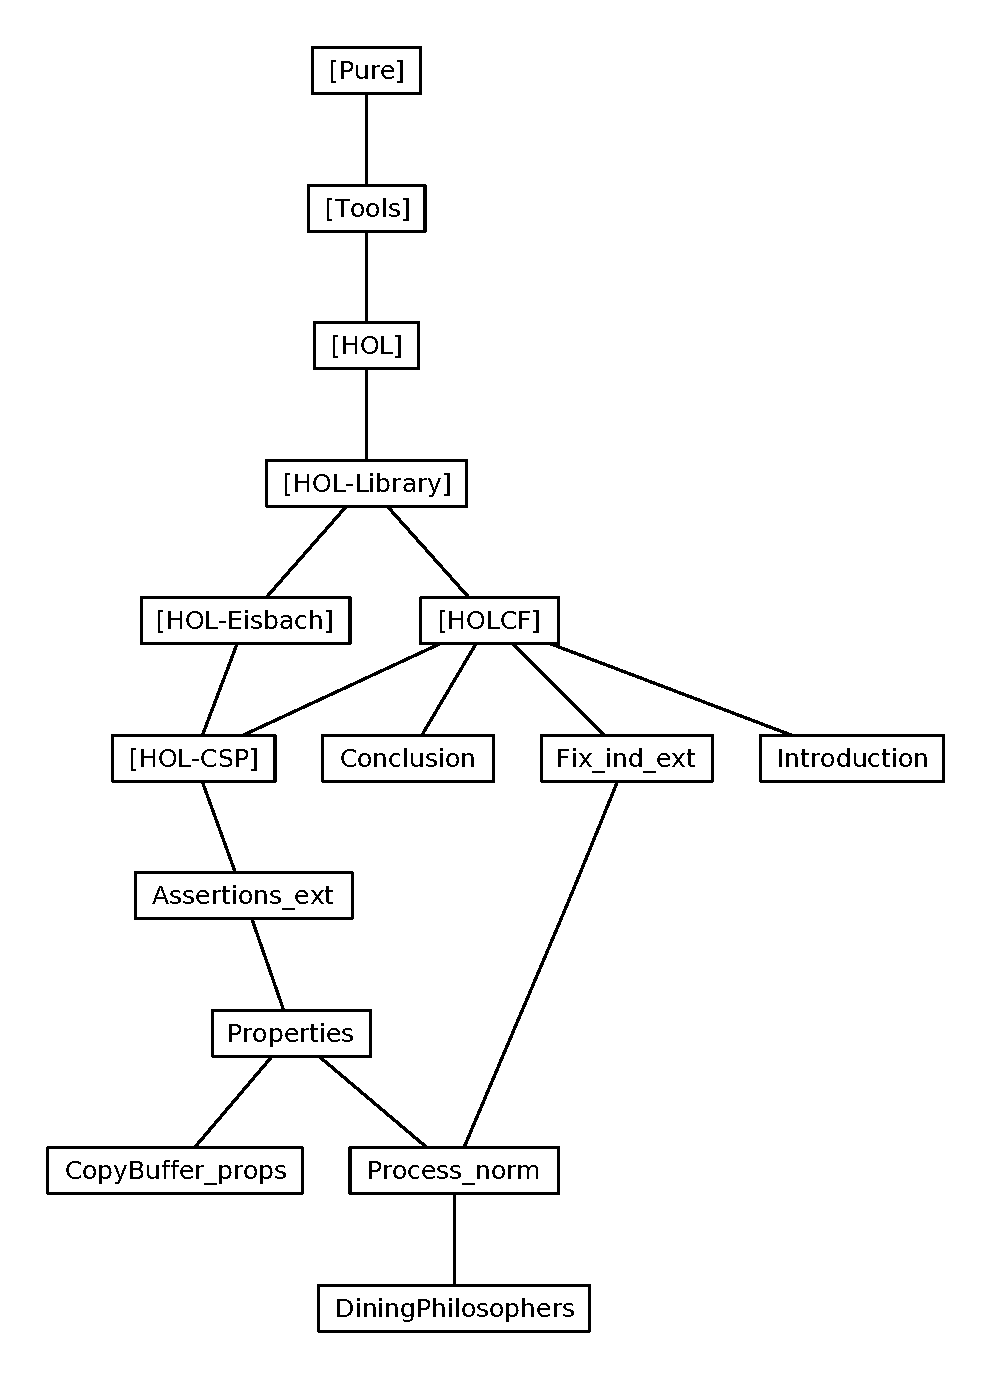
\includegraphics[height=\textheight]{session_graph}}
  \caption{The Dependency Graph of the Isabelle Theories.\label{fig:session-graph}}
\end{sidewaysfigure}

\nocite{foster.ea:efsm:2018}

\clearpage

\input{session}


{\small
  \bibliographystyle{abbrvnat}
  \bibliography{root}
}
\end{document}
\endinput

%%% Local Variables:
%%% mode: latex
%%% TeX-master: t
%%% End:
